\documentclass[twoside,letterpaper]{soups-poster} 
\pdfpagewidth=8.5truein 
\pdfpageheight=11truein 

\usepackage{graphicx}
\usepackage{float}
\usepackage{subfloat}
\usepackage{caption}
\usepackage[usenames,dvipsnames]{xcolor}
\usepackage{multirow}


\definecolor{darkred}{HTML}{E50000}

\renewcommand{\topfraction}{0.99} % be more aggressive about text around floats
\renewcommand{\floatpagefraction}{0.99}
\pagestyle{plain}

\begin{document}
%
% --- Author Metadata here ---
%\conferenceinfo{Symposium on Usable Privacy and Security(SOUPS)}{2010, July 14--16, 2009, Redmond, WA, USA}
%\CopyrightYear{2010} % Allows default copyright year (200X) to be over-ridden - IF NEED BE.
%\crdata{0-12345-67-8/90/01}  % Allows default copyright data (0-89791-88-6/97/05) to be over-ridden - IF NEED BE.
% --- End of Author Metadata ---

\title{Poster: Clarity of Facebook Connect login permissions}

\numberofauthors{2} 
\author{
\alignauthor
Nicky Robinson\\
       \affaddr{Princeton University}\\
       \email{ncrobins@princeton.edu}
% 2nd. author
\alignauthor
Joseph Bonneau\\
       \affaddr{Princeton University}\\
       \email{jbonneau@princeton.edu}
}

\maketitle


\section{Introduction}
Single Sign-On (SSO) systems allow users to log in to websites using their username and password from a third-party identity provider.
This means fewer passwords for users to remember which theoretically means they can create more complicated and therefore more secure passwords.

Facebook Connect, based off of OAuth, is perhaps the most common SSO system.
It does more than just allow a user to sign in: sites can request access to parts of the user's Facebook profile.
When the developer integrates the login system with their website, they request various permissions from Facebook to read information from the user's profile or publish content to their profile. %The permissions available to the developer can be seen in the Facebook Connect documentation \cite{fbpermissions}.

Users logging in with Facebook Connect place a lot of trust in Facebook to only share information that the user authorizes.
This relies both on Facebook granting only the permissions presented in the authorization messages and users correctly interpreting these messages.
We explored user understanding of authorization messages via an online survey conducted over Amazon Mechanical Turk presenting users with Facebook permissions dialogues and asking them to identify which permissions would be granted if they approved the applications.
We identified a number of areas where user understanding is inconsistent with the mechanics of Facebook Connect.
In general, users believe that Facebook Connect authorizes far less information to be shared than it actually authorizes.

\section{Read vs. write permissions}

While experimenting with Facebook Connect and crawling sites which deploy it for authentication, we discovered that while developers may request read permissions for individual items in a user's profile on a granular basis, write permission are all-or-nothing.
If the developer requests any write permissions, Facebook shows the user a generic message saying that the app is requesting permission to ``post to Facebook for you.'' If the user clicks okay, the site will receive all write permissions.
We communicated with Facebook Security and confirmed that this was not a bug but a design decision to make the messages easier to understand.

To test whether it is actually easier to understand, we conducted a survey with 600 respondents.
We presented half with Facebook's standard write permissions message followed by 13 options of things they might be giving the site permission to do by clicking okay. Eight of the 13 were taken almost directly from the Facebook Connect documentation's permission descriptions \cite{fbpermissions}, so they were all things the site would be able to do (since Facebook gives all write permissions together). The other five were things the site could not do. They were present not to be tested but to eliminate biases due to an aversion to selecting all available options. 
The other half were presented with read permissions questions.
Since read permissions messages vary, we used messages taken from four different real sites with varying numbers of permissions (\emph{Jabong.com}, \emph{Flickr.com}, \emph{Splashscore.com}, and \emph{TripAdvisor.com}).
All were renamed ``Hooli.com.''
Each message was followed with eight or nine options for things the site might be able to do. Four or five options were information on a Facebook profile that the site would be able to see. The other four were either things the site could not see or were write or extended permissions. Again, the incorrect answers were only so the respondent did not have to select all options to be correct. There are too many different read permissions to effectively test them all without exhausting the respondents with too many questions, so the ones tested are some of the more common ones.

Our null hypothesis was that users would not be any more or less accurate at determining which read permission were being granted vs. write permissions.
Our results are shown in Figure~\ref{figure:readpercents} and Figure~\ref{figure:writepercents}. 
For all tested read permissions, over half of people correctly identified that said permission would be granted based on the message presented.
On average, individual permissions were correctly identified 79.72\% of the time, comparable to previous research~\cite{egelman}.

\begin{figure}[tbh!]
  \centering
  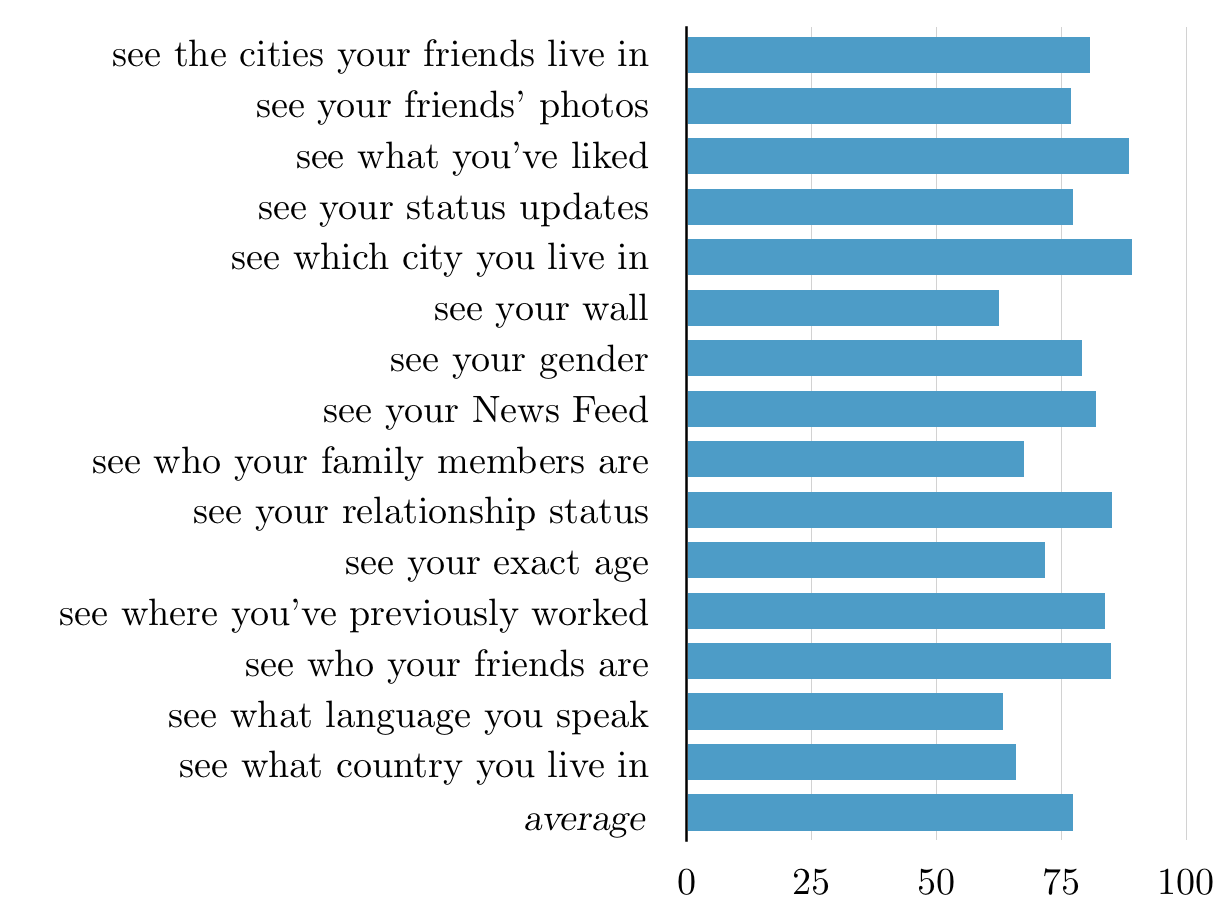
\includegraphics[width=8.5cm]{read_percents_cosn}
  \caption{Percentage of respondents who correctly identified that each read permission would be granted upon approval.}
  \label{figure:readpercents}
\end{figure}

\begin{figure}[h!]
  \centering
  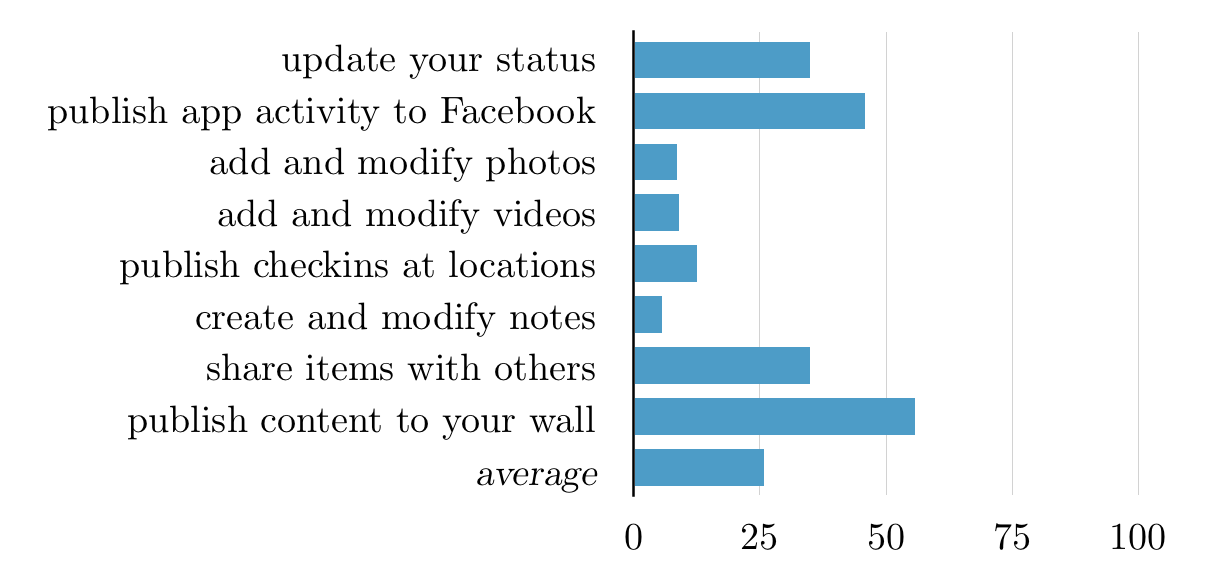
\includegraphics[width=8.5cm]{write_percents_cosn}
  \caption{Percentage of respondents who correctly identified that each write permission would be granted upon approval.}
  \label{figure:writepercents}
\end{figure}

However, write permissions were only correctly identified 25.91\% of the time, signicificantly worse than if users were randomly guessing.
Using A Mann-Whitney $U$ test to compare the average understanding of users these two groups allows us to reject the null hypothesis with $p < 0.001$ and conclude that users understand read permissions significantly more accurately than they do write permissions.


\section{Reading non-public data}

In one pilot study we conducted a respondent stated that the requesting site would gain access to only a limited amount of data because their Facebook privacy settings made the rest not visible.
This suggests a lack of understanding of how the read permissions work: upon granting the site read permissions, the site can access that information regardless of the user's privacy settings.

We surveyed 100 participants to test if this confusion was widespread. The survey presented the user with the permission message for \emph{Imgur.com}, which requests the \emph{user\_photos} permission. Users were asked to identify which photo albums Imgur would be able to see if they clicked okay. The options were those marked as visible to the public, those marked as visible to friends, and those marked as visible to only them. All three options are in fact correct.
Our null hypothesis is that users would be equally likely to identify that data could be read regardless of its privacy setting.

Results are shown in Figure~\ref{figure:privacypercents}. A G-test allows us to reject the null hypothesis with $p < .001$.
It appears people are generally aware that they are giving access to their photo albums that are marked as public but are unaware that they are also giving access to their photo albums that are marked as visible to their friends or only to themselves.
This suggests that the relatively high comprehension levels found in our previous survey (79.72\%) and Egelman's study (88\%) \cite{egelman} may not actually be entirely representative of user understanding: although people know which types of information they are granting access to, most do not realize they are giving access to that information even if they have marked it with a privacy level other than public. However, this section of our study was performed on a relatively small scale (one website with one permission and 100 responses).

\begin{figure}[h!]
  \centering
  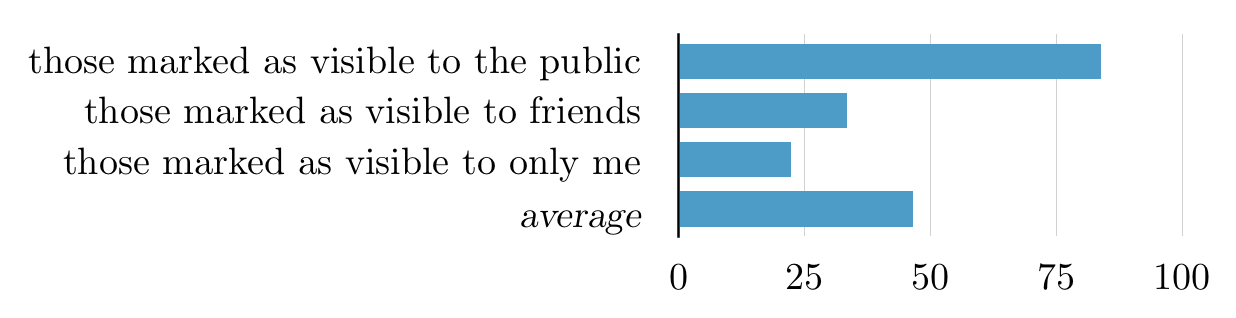
\includegraphics[width=8.5cm]{privacy_percents_cosn}
  \caption{Percentage of respondents who correctly identified that Imgur.com would be able to see their photo albums of each privacy level upon authorization.}
  \label{figure:privacypercents}
\end{figure}

\section{Influence of requesting site}

Our pilot participants also indicated that the site requesting the permissions may influence how they interpret the write permissions message. 
We surveyed 300 separate participants to test this. The format of the survey was identical to the write permissions questions in the first survey and we provided the same options for the user to select. However, instead of using ``Hooli.com'' as the website in question, one third of respondents were presented with \emph{Flickr.com} (a photo and video sharing site), one third with \emph{TripAdvisor.com} (a travel site), and one third with \emph{iFlikeU.com} (an anonymous messaging site).

Figure~\ref{figure:multipercents} illustrates the percentage of people who correctly identified that each permission would be given to each site after they clicked okay.

\begin{figure}[h!]
  \centering
  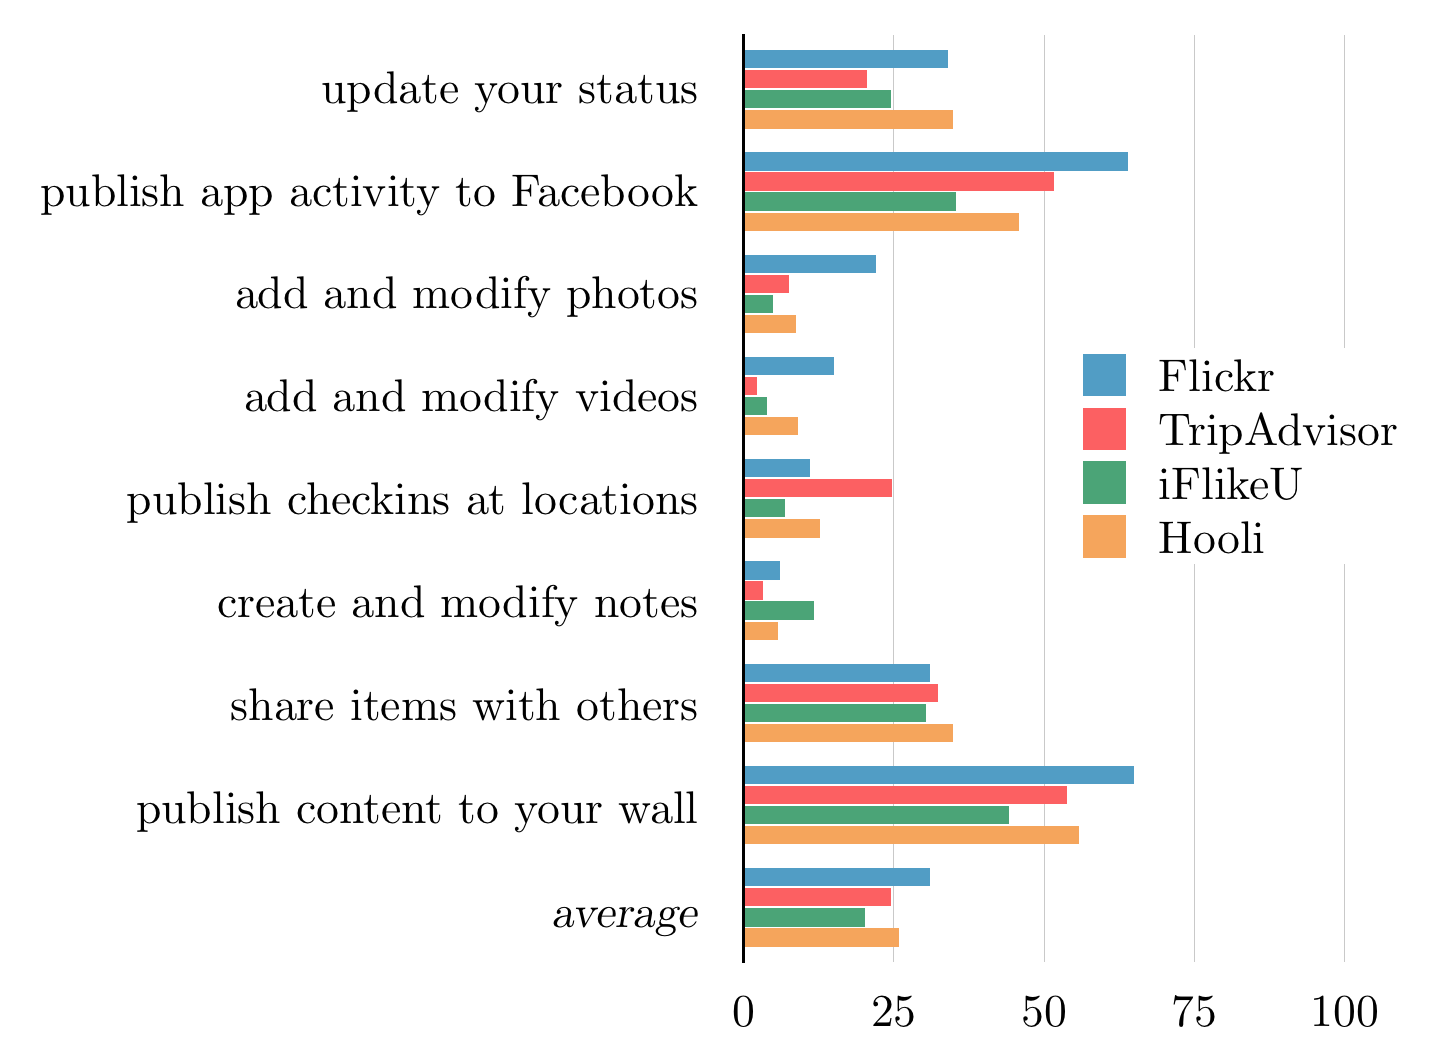
\includegraphics[width=8.5cm]{multi_percents_cosn}
  \caption{Percent of respondents who correctly identified which permissions would be granted for each requesting site.}
  \label{figure:multipercents}
\end{figure}

For ``publish app activity to Facebook,'' ``add and modify photos,'' ``add and modify videos,'' and ``publish checkins at locations,'' the null hypothesis (that the site identity does not affect how many people think a given permission is being requested) can be rejected with $p < .01$ using a $G$-test. More respondents thought Flickr would be able to add and modify photos and videos compared to other sites, which is reasonable since it is a photo and video sharing site. Likewise, many more people thought that TripAdvisor would be able to publish checkins at locations---a logical thing for a travel site to do.
It appears that users' perception of the write permissions message is influenced by the site identity for some permissions.

\bibliographystyle{abbrv}
\bibliography{report_references}  
\end{document}
